\documentclass[25pt, a0paper, portrait, margin=0mm,
innermargin=15mm]{tikzposter}
\usepackage{wrapfig,kantlipsum}
\usepackage{hyperref}

\title{Title}
\author{Name}
\institute{University}
\usetheme{Default}
\usecolorstyle[colorPalette=BrownBlueOrange]{Germany}
%\usepackage{graphicx}%<= Tikz loads this so no need.

\begin{document}
\maketitle

\begin{columns}
\column{.5}
       \block{Methods}{
          We collected tweets using the public Twitter Streaming RESTful API
          over 2014-10-15 \textemdash 2014-11-09 by tracking words that related
          to various tech stocks indexed by NASDAQ.           
          \innerblock{Examples of Tweets}{
          \begin{itemize}
            \item \small{Maine nurse defies Ebola quarantine order by taking bike ride.
              http://t.co/eERINkm3AQ via @indystarJ}
            \item \small{Tim Cook: Apple CEO Says 'Being Gay Is One Of God's
                Greatest Gifts' Earlier today, the chief executive of
                Apple,\ldots \url{http://t.co/zIXb2HbDmd}}
            \item \small{ Meet the Swedish twin sisters who want to be
                'identical artificial dolls' \url{http://t.co/77eA3esaQa}}
            \item \small{Last Christmas I got a black iPhone it was the
                worst Christmas present ever, I wanted a white one. I mean I'm
                not\ldots \url{http://t.co/jhP9ODs3QK}}
            \end{itemize}
          }
          \innerblock{Kewords tracked}{
            \begin{itemize}\label{keywords}
            \item \small{ 'ebola', 'aapl', 'apple', 'mac', 'tim cook', 'goog',
            'google', 'gmail', 'youtube', 'microsoft', 'msft',
            'nadella', 'twrt', 'amazon', 'amzn', 'prime', 'aws','fb',
          'facebook'}
          \end{itemize}
        }
       \begin{wrapfigure}[12]{r}{0.35\linewidth}
           \begin{tikzfigure}[Rolling sample.] \label{fig:rollingmeans}
             %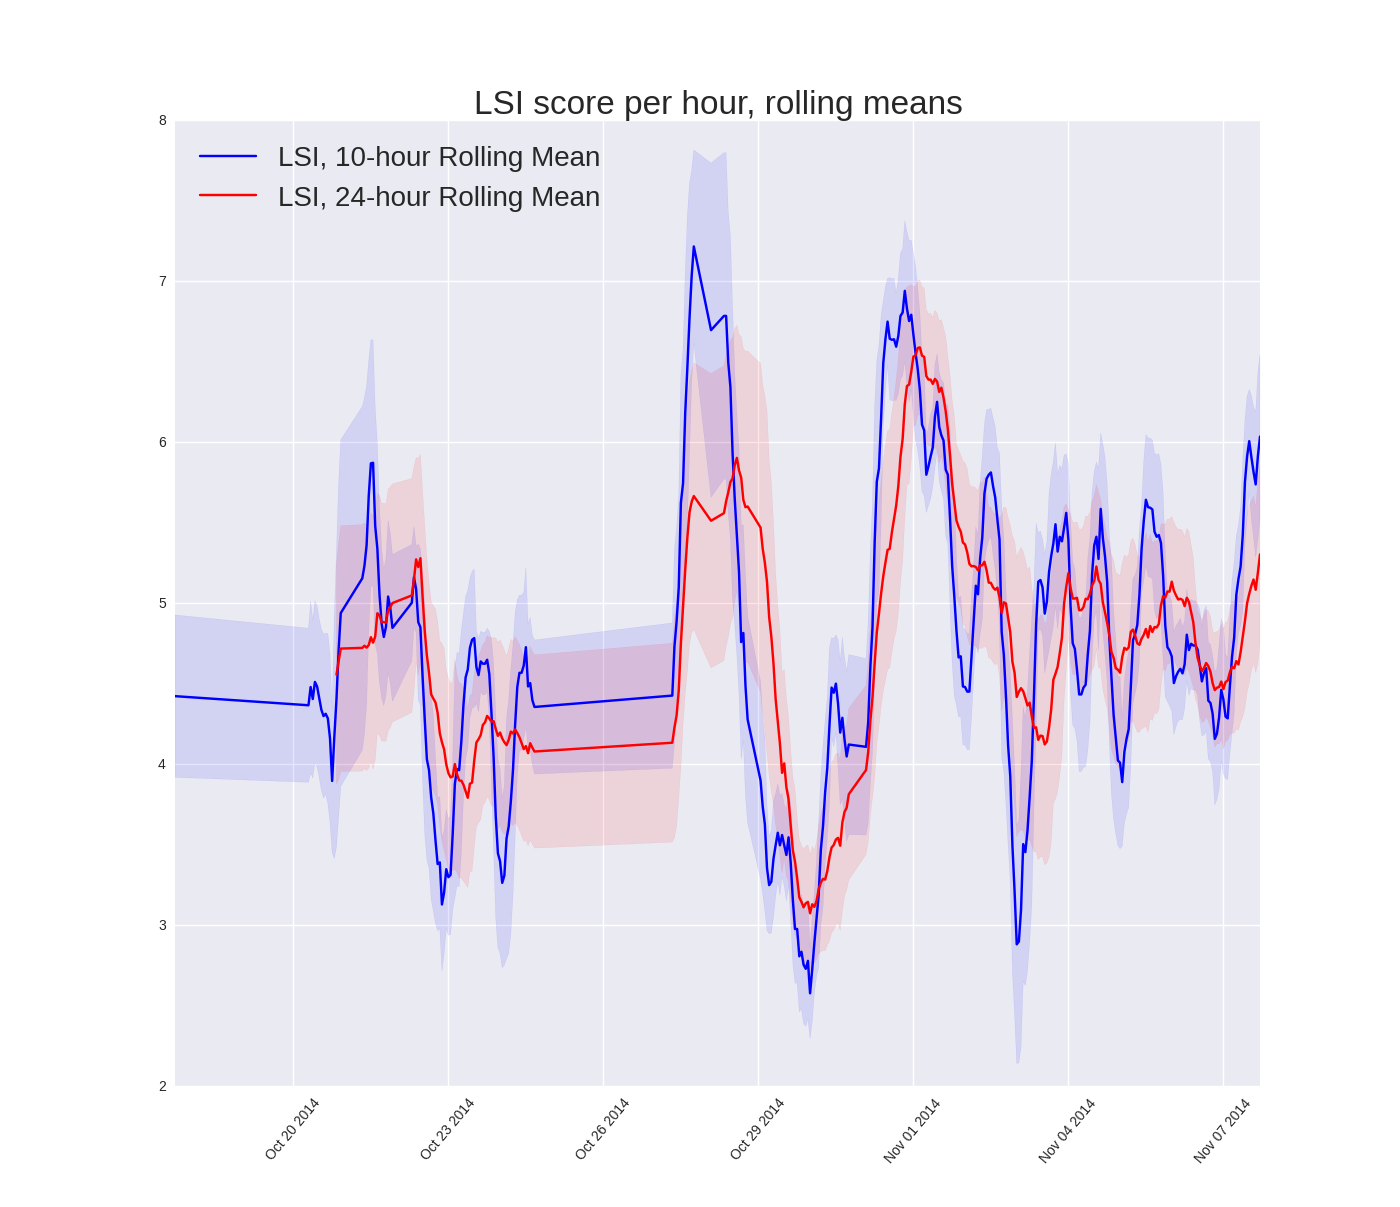
\includegraphics[width=4in]{figures/lsi_rolling_means.png}
             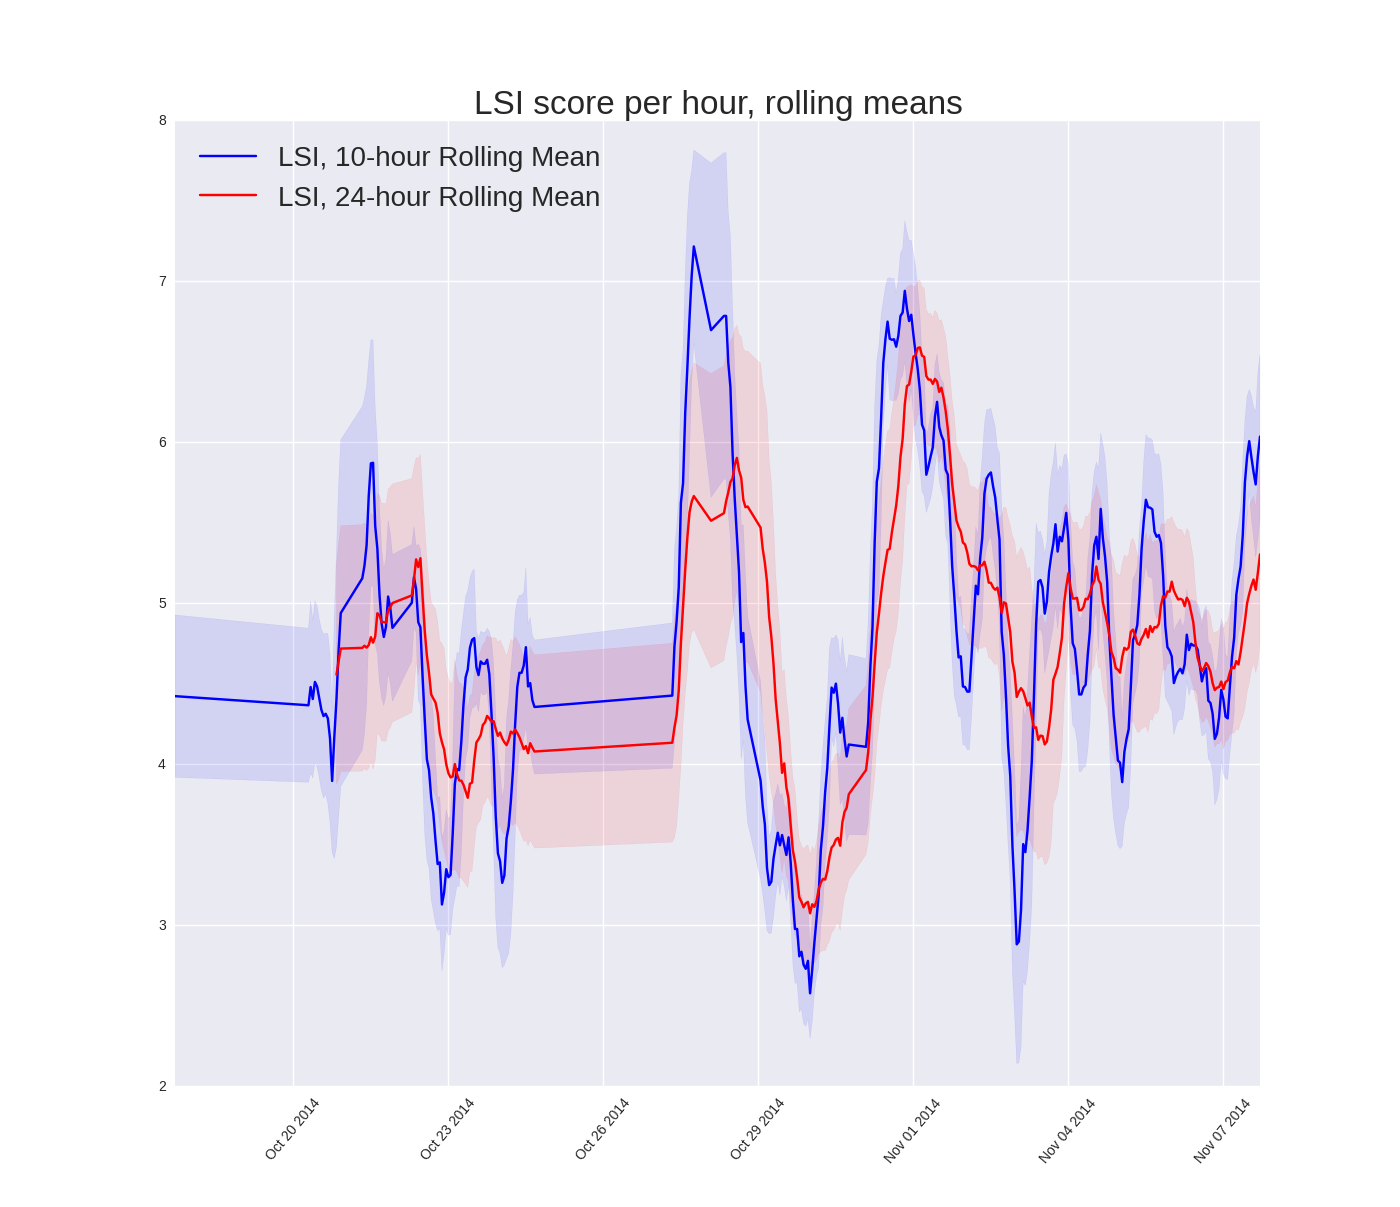
\includegraphics[width=9cm]{figures/lsi_rolling_means.png}
           \end{tikzfigure}
         \end{wrapfigure}
          NASDAQ market data was also
          collected over the same period. Tweets were preprocessed to remove
          common stopwords and latent semantic indexing was performed on
          one-hour bag-of-words bins of tweets, giving a total of xxx hours
          included in analysis. Each hour bin's LSI topics were scored using
          the AFINN database, resulting in a single number indicating semantic
          valence for each hour. This semantic data was combined with the stock
          data for visualization and analysis. A vector autoregressive (VAR)
          model was performed to assess the predictive power of the semantic
          data against the stock data.
          
     }

\block[roundedcorners=40]{First block}{
  \kant[1-2]

  \begin{wrapfigure}[12]{r}{0.5\linewidth}
    \begin{tikzfigure}[Caption]
      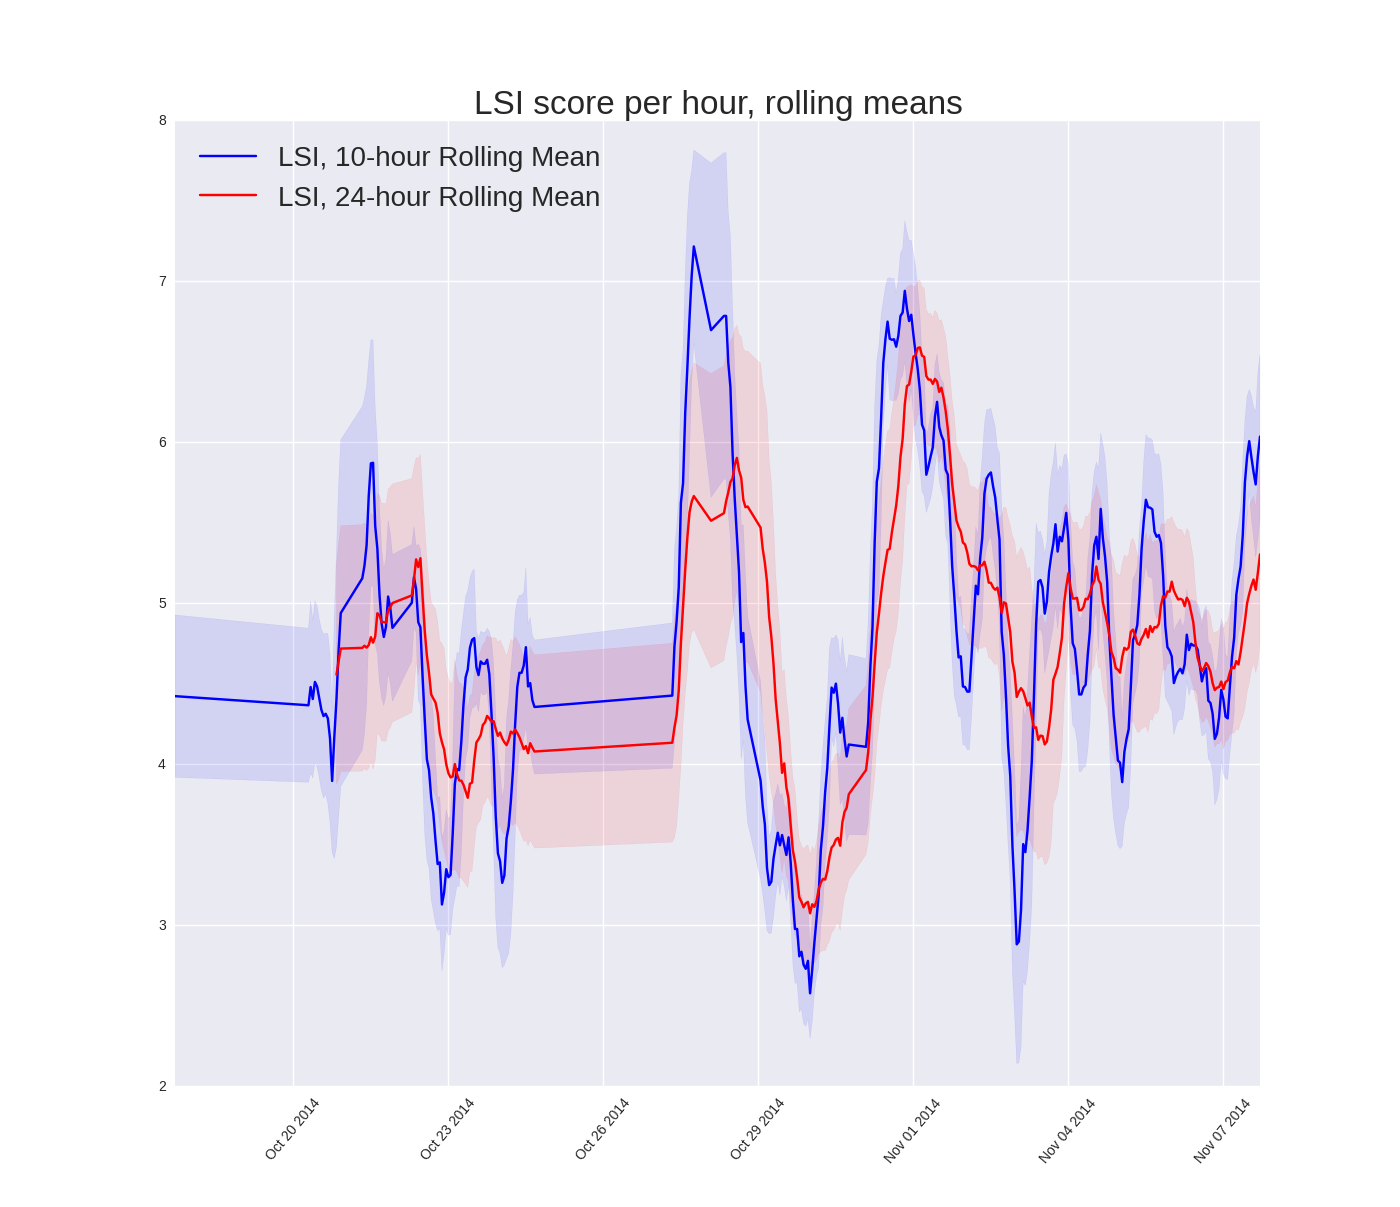
\includegraphics[width=4cm]{figures/lsi_rolling_means.png}
    \end{tikzfigure}
  \end{wrapfigure}

  \kant[1]
}
\end{columns}
\end{document}
